\documentclass[journal,12pt,twocolumn]{IEEEtran}
\usepackage{setspace}
\usepackage{gensymb}
\usepackage{xcolor}
\usepackage{caption}
\singlespacing
\usepackage{siunitx}
\usepackage[cmex10]{amsmath}
\usepackage{mathtools}
\usepackage{hyperref}
\usepackage{amsthm}
\usepackage{mathrsfs}
\usepackage{txfonts}
\usepackage{stfloats}
\usepackage{cite}
\usepackage{cases}
\usepackage{subfig}
\usepackage{longtable}
\usepackage{multirow}
\usepackage{enumitem}
\usepackage{mathtools}
\usepackage{listings}
\usepackage{tikz}
\usetikzlibrary{shapes,arrows,positioning}
\usepackage{circuitikz}
\let\vec\mathbf
\DeclareMathOperator*{\Res}{Res}
\renewcommand\thesection{\arabic{section}}
\renewcommand\thesubsection{\thesection.\arabic{subsection}}
\renewcommand\thesubsubsection{\thesubsection.\arabic{subsubsection}}

\renewcommand\thesectiondis{\arabic{section}}
\renewcommand\thesubsectiondis{\thesectiondis.\arabic{subsection}}
\renewcommand\thesubsubsectiondis{\thesubsectiondis.\arabic{subsubsection}}
\hyphenation{op-tical net-works semi-conduc-tor}

\lstset{
language=Python,
frame=single, 
breaklines=true,
columns=fullflexible
}
\begin{document}
\theoremstyle{definition}
\newtheorem{theorem}{Theorem}[section]
\newtheorem{problem}{Problem}
\newtheorem{proposition}{Proposition}[section]
\newtheorem{lemma}{Lemma}[section]
\newtheorem{corollary}[theorem]{Corollary}
\newtheorem{example}{Example}[section]
\newtheorem{definition}{Definition}[section]
\newcommand{\BEQA}{\begin{eqnarray}}
\newcommand{\EEQA}{\end{eqnarray}}
\newcommand{\define}{\stackrel{\triangle}{=}}
\newcommand{\myvec}[1]{\ensuremath{\begin{pmatrix}#1\end{pmatrix}}}
\newcommand{\mydet}[1]{\ensuremath{\begin{vmatrix}#1\end{vmatrix}}}
\bibliographystyle{IEEEtran}
\providecommand{\nCr}[2]{\,^{#1}C_{#2}} % nCr
\providecommand{\nPr}[2]{\,^{#1}P_{#2}} % nPr
\providecommand{\mbf}{\mathbf}
\providecommand{\pr}[1]{\ensuremath{\Pr\left(#1\right)}}
\providecommand{\qfunc}[1]{\ensuremath{Q\left(#1\right)}}
\providecommand{\sbrak}[1]{\ensuremath{{}\left[#1\right]}}
\providecommand{\lsbrak}[1]{\ensuremath{{}\left[#1\right.}}
\providecommand{\rsbrak}[1]{\ensuremath{{}\left.#1\right]}}
\providecommand{\brak}[1]{\ensuremath{\left(#1\right)}}
\providecommand{\lbrak}[1]{\ensuremath{\left(#1\right.}}
\providecommand{\rbrak}[1]{\ensuremath{\left.#1\right)}}
\providecommand{\cbrak}[1]{\ensuremath{\left\{#1\right\}}}
\providecommand{\lcbrak}[1]{\ensuremath{\left\{#1\right.}}
\providecommand{\rcbrak}[1]{\ensuremath{\left.#1\right\}}}
\theoremstyle{remark}
\newtheorem{rem}{Remark}
\newcommand{\sgn}{\mathop{\mathrm{sgn}}}
\newcommand{\rect}{\mathop{\mathrm{rect}}}
\newcommand{\sinc}{\mathop{\mathrm{sinc}}}
\providecommand{\abs}[1]{\left\vert#1\right\vert}
\providecommand{\res}[1]{\Res\displaylimits_{#1}} 
\providecommand{\norm}[1]{\lVert#1\rVert}
\providecommand{\mtx}[1]{\mathbf{#1}}
\providecommand{\mean}[1]{E\left[ #1 \right]}
\providecommand{\fourier}{\overset{\mathcal{F}}{ \rightleftharpoons}}
\providecommand{\ztrans}{\overset{\mathcal{Z}}{ \rightleftharpoons}}
\providecommand{\system}[1]{\overset{\mathcal{#1}}{ \longleftrightarrow}}
\newcommand{\solution}{\noindent \textbf{Solution: }}
\providecommand{\dec}[2]{\ensuremath{\overset{#1}{\underset{#2}{\gtrless}}}}
\let\StandardTheFigure\thefigure
\def\putbox#1#2#3{\makebox[0in][l]{\makebox[#1][l]{}\raisebox{\baselineskip}[0in][0in]{\raisebox{#2}[0in][0in]{#3}}}}
     \def\rightbox#1{\makebox[0in][r]{#1}}
     \def\centbox#1{\makebox[0in]{#1}}
     \def\topbox#1{\raisebox{-\baselineskip}[0in][0in]{#1}}
     \def\midbox#1{\raisebox{-0.5\baselineskip}[0in][0in]{#1}}

\vspace{3cm}
\title{Line Assignment}
\author{Gautam Singh}
\maketitle
\bigskip

\begin{abstract}
    This document contains the solution to Question 16 of Exercise 2 in Chapter
    11 of the class 12 NCERT textbook.
\end{abstract}

\begin{enumerate}
    \item Find the shortest distance between the lines whose vector equations are
    \begin{align}
        \vec{r} = \myvec{1\\2\\3} + \lambda\myvec{1\\-3\\2}
        \label{eq:L1}
    \end{align}
    and
    \begin{align}
        \vec{r} = \myvec{4\\5\\6} + \mu\myvec{2\\3\\1}
        \label{eq:L2}
    \end{align}

    \solution The shortest distance between the two lines would be along the 
    vector normal to both direction vectors. The given direction vectors are
    \begin{align}
        \vec{A} = \myvec{1\\-3\\2} \qquad \vec{B} = \myvec{2\\3\\1}
        \label{eq:dir-vec}
    \end{align}
    Hence, their cross product is
    \begin{align}
        \vec{C} = \vec{A}\times\vec{B} &= \myvec{\mydet{\vec{A_{23}}&\vec{B_{23}}}\\
                                                \mydet{\vec{A_{31}}&\vec{B_{31}}}\\
                                                \mydet{\vec{A_{12}}&\vec{B_{12}}}
                                                } \\
        &= \myvec{\mydet{-3&3\\2&1}\\\mydet{2&1\\1&2}\\\mydet{1&2\\-3&3}} = \myvec{-9\\3\\9}                
        \label{eq:cross-prod}
    \end{align}
    where
    \begin{align}
        \vec{P_{ij}} \define \myvec{p_i\\p_j}
        \label{eq:def-Aij}
    \end{align}
    From \eqref{eq:L1} and \eqref{eq:L2}, the points on the first and second 
    line respectively are
    \begin{align}
        \vec{P} = \myvec{1\\2\\3} \qquad \vec{Q} = \myvec{4\\5\\6}
        \label{eq:pts}
    \end{align}
    Hence, the vector joining $\vec{P}$ and $\vec{Q}$ is given by
    \begin{align}
        \vec{D} = \vec{Q} - \vec{P} = \myvec{3\\3\\3}
    \end{align}
    Therefore, the magnitude of the vector component of $\vec{D}$ along 
    $\vec{C}$ is the required shortest distance, and is given by
    \begin{align}
        d &= \frac{\norm{\vec{C}^\top\vec{D}}}{\norm{\vec{C}}} \\
          &= \frac{9}{\sqrt{(-9)^2+3^2+9^2}} \\
          &= \frac{3}{\sqrt{13}}\ \textrm{units}
          \label{eq:dist}
    \end{align}
    The situation is depicted in Fig. \ref{fig:plot-3d}, which is generated using 
    the Python code \texttt{codes/plot\_3d.py}.
    \begin{figure}[!ht]
        \centering
        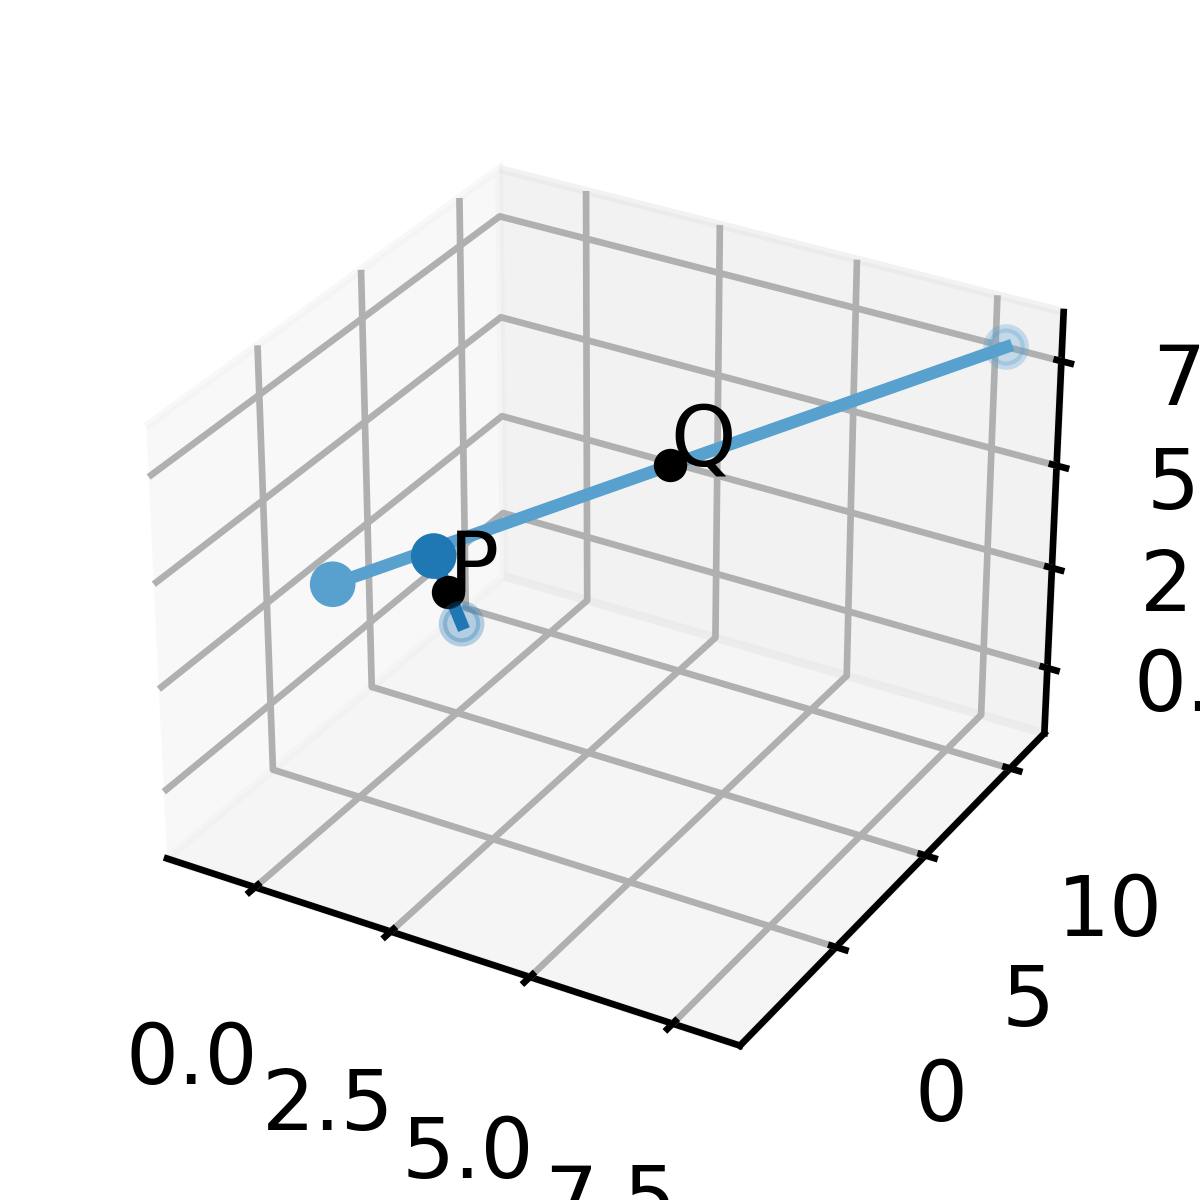
\includegraphics[width=\columnwidth]{figs/plot_3d.png}
        \caption{Finding the shortest distance between two skew lines.}
        \label{fig:plot-3d}
    \end{figure}
\end{enumerate}
\end{document}
